\documentclass[11pt]{article}

% ====================================================
% ====================================================
% USEPACKAGES AND IMPORTS
% ====================================================
% ====================================================

\usepackage[T1]{fontenc}
\usepackage[utf8]{inputenc}
\usepackage[english]{babel}

\usepackage{fancyhdr}

% definitions
% ====================================================
\let\titleoriginal\title
\renewcommand{\title}[1]{
	\titleoriginal{#1}
	\newcommand{\thetitle}{#1}
}

\setlength{\parskip}{\baselineskip}%
\setlength{\parindent}{0pt}%

% header and footer
\pagestyle{fancy}
\fancyhf{}
\lhead{Applied Machine Learning Fundamentals}
\rhead{\thetitle}
\cfoot{\thepage}

% ====================================================
% ====================================================
% PRESENTATION DATA
% ====================================================
% ====================================================

\title[Deep Learning]{*** Applied Machine Learning Fundamentals *** Neural Networks / Deep Learning}
\institute{SAP\,SE}
\author{Clemens Biehl, Daniel Wehner}
\date{Winter term 2019/2020}
\prefix{DL}

% ====================================================
% ====================================================
% BEGIN OF DOCUMENT
% ====================================================
% ====================================================

\begin{document}

% Title frame
%______________________________________________________________________
\maketitlepage


% Lecture Overview
%______________________________________________________________________
\begin{frame}{Lecture Overview}{}
	\makeoverview{8}
\end{frame}


% Agenda
%______________________________________________________________________
\begin{frame}{Agenda for this Unit}
	\begin{multicols}{2}
		\tableofcontents
	\end{multicols}
\end{frame}


% Section: Introduction
%______________________________________________________________________
\section{Introduction}
\makedivider{Introduction}

% Subsection: What is Deep Learning?
% --------------------------------------------------------------------------------------------------------
\subsection{What is Deep Learning?}

% What is Deep Learning?
\begin{frame}{What is Deep Learning?}{}
	\begin{itemize}
		\item `Deep Learning' is a fancy new term for `artificial neural networks' 
		\item It is a \textbf{supervised} method and \textbf{model based}
		\item Artificial neural networks are inspired by the human brain
		\item Lots of different architectures exist:
		\begin{itemize}
			\item \highlight{Multi-Layer perceptrons (MLPs)}
			\item \highlight{Convolutional neural networks (CNNs, ConvNets)}
			\item \highlight{Recurrent neural networks (LSTMs, GRUs, etc.)}
			\item ...and many more...
		\end{itemize}
	\end{itemize}
\end{frame}


% Subsection: History of Deep Learning?
% --------------------------------------------------------------------------------------------------------
\subsection{History of Deep Learning}

% History of Deep Learning
\begin{frame}{History of Deep Learning}{}
	\footnotesize
	\divideTwo{0.49}{
		\begin{boxBlueNoFrame}
			\textbf{Early booming} (1950s -- early 1960s) \\

			\textit{F. Rosenblatt} suggests the \highlight{Perceptron} learning algorithm:
				\href{https://blogs.umass.edu/brain-wars/files/2016/03/rosenblatt-1957.pdf}{\linkstyle{Click here!}}
		\end{boxBlueNoFrame}
	}{0.49}{
		\begin{boxBlueNoFrame}
			\begin{figure}
				\centering
				\includegraphics[scale=0.875]{10_deep_learning/02_img/perceptron_rosenblatt}
			\end{figure}
		\end{boxBlueNoFrame}
	}

	\divideTwo{0.49}{
		\begin{boxBlueNoFrame}
			\begin{figure}
				\centering
				\includegraphics[scale=0.19]{10_deep_learning/02_img/perceptron_xor}
			\end{figure}
		\end{boxBlueNoFrame}
	}{0.49}{
		\begin{boxBlueNoFrame}
			\textbf{Setback I} (mid 1960s -- late 1970s) \\

			\textit{M.\,Minsky} and \textit{S.\,Papert} (1969): \\
			Serious problems with perceptron algorithm:
			It cannot learn the \textbf{XOR problem}.
		\end{boxBlueNoFrame}
	}
\end{frame}


% History of Deep Learning (Ctd.)
\begin{frame}{History of Deep Learning (Ctd.)}{}
	\footnotesize
	\divideTwo{0.49}{
		\begin{boxBlueNoFrame}
			\textbf{Renewed enthusiasm} (1980s)
			\begin{itemize}
				\setlength\itemsep{0.15em}
				\item New techniques available
				\item \highlight{Backpropagation} for deep nets
			\end{itemize}	
		\end{boxBlueNoFrame}

		\begin{boxBlueNoFrame}
			\textbf{Setback II} (1990s -- mid 2000s)
			\begin{itemize}
				\setlength\itemsep{0.15em}
				\item Other techniques were considered superior (e.\,g. SVMs)
				\item CS journals rejected papers on neural networks
			\end{itemize}
		\end{boxBlueNoFrame}
	}{0.49}{
		\begin{boxBlue}
			\textbf{`Deep Learning'} (since mid 2000) \\ \vspace*{1mm}

			More data, faster computers, better optimization techniques...

			\begin{figure}
				\centering
				\includegraphics[scale=0.275]{10_deep_learning/02_img/deep_learning}
			\end{figure}
		\end{boxBlue}
	}
\end{frame}


% Subsection: Biological Motivation
% --------------------------------------------------------------------------------------------------------
\subsection{Biological Motivation}

% Biological Motivation
\begin{frame}{Biological Motivation}{}
	\begin{itemize}
		\item All neurons are connected and form a complex \textbf{network}
		\item \textbf{Transmitter chemicals} within the fluid of the brain influence the
			\textbf{electrical potential} inside the body of the neurons
		\item If the \textbf{membrane potential} reaches some threshold, the neurons \textbf{fires} \\
			$\Rightarrow$ A pulse of fixed length is sent down the \textbf{axon}
		\item The axon connects the neuron with other neurons (via \textbf{synapses})
		\item Probably there are 100 trillion \textcolor{red}{\textbf{(!!!)}} synapses in the human brain
		\item \textbf{Refractory period} after a neuron has fired
	\end{itemize}
\end{frame}


% Biological Motivation (Ctd.)
\begin{frame}[plain]{}{}
	\begin{figure}
		\centering
		\includegraphics[scale=0.50]{10_deep_learning/02_img/biological_neuron}
	\end{figure}
\end{frame}


% How can we know this?
\begin{frame}{How can we know this?}{}
	\divideTwo{0.29}{
		\begin{figure}
			\centering
			\includegraphics[scale=0.15]{10_deep_learning/02_img/cajal_golgi_stain}
		\end{figure}
	}{0.69}{
		\footnotesize
		\begin{itemize}
			\item \textit{Santiago Ramón y Cajal} made neurons visible by applying \textbf{Golgi's method}
			\item Golgi's method uses the \textbf{Golgi stain} to colorize the neurons
		\end{itemize}
	} \\
	\vspace*{3mm}
	\divideTwo{0.59}{
		\footnotesize
		\begin{itemize}
			\item End of the 1940s, \textit{Hodgkin} and \textit{Huxley} started investigating the electrical properties of
				neurons on the squid's axon
			\item The right-hand-side image was the first \textbf{action potential} ever plotted
		\end{itemize}
	}{0.39}{
		\begin{figure}
			\centering
			\includegraphics[scale=0.3]{10_deep_learning/02_img/spike_potential_squid}
		\end{figure}
	}
\end{frame}


% How do Humans / Animals learn?
\begin{frame}{How do Humans / Animals learn?}{}
	\footnotesize
	\vspace*{-2mm}
	\begin{itemize}
		\item \textbf{Idea:} Mechanism of learning is \highlight{association}
		\item \highlight{Hebbian learning:} If the firing of one neuron repeatedly assists in firing another neuron,
			the synaptic connection will be strengthened
	\end{itemize}
	
	\begin{boxBlueNoFrame}
		\textit{`When an axon of cell A is near enough to excite a cell B and repeatedly or persistently \textbf{takes part in
			firing it}, some growth process or \textbf{metabolic change} takes place in one or both cells such that
			A's \textbf{efficiency}, as one of the cells firing B, is \textbf{increased}.'} \\[-3mm]

		\textit{`The general idea is an old one, that any two cells or systems of cells that are
			\textbf{repeatedly active at the same} time will tend to become \textbf{`associated'}, so that activity
			in one facilitates activity in the other.'} \hfill \textit{Hebb}
	\end{boxBlueNoFrame}
\end{frame}


% Classical / Pavlovian Conditioning
\begin{frame}{Classical / Pavlovian Conditioning}{}
	\footnotesize
	\divideTwo{0.55}{
		\begin{itemize}
			\item Dog salivates when given food
			\item Food is an \highlight{unconditioned stimulus (US)}
			\item Salivation in response to food is \highlight{unconditioned response (UR)}
			\item Food is paired with the sound of a bell
			\item Bell is  \highlight{conditioned stimulus (CS)}
			\item Bell will eventually elicit salivation event without food
			\item Salivation is  \highlight{conditioned response (CR)}
		\end{itemize}
	}{0.43}{
		\begin{figure}
			\centering
			\includegraphics[scale=0.50]{10_deep_learning/02_img/pavlov}
		\end{figure}
	}
\end{frame}


% Classical / Pavlovian Conditioning (Ctd.)
\begin{frame}{Classical / Pavlovian Conditioning (Ctd.)}{}
	\begin{figure}
		\centering
		\includegraphics[scale=0.70]{10_deep_learning/02_img/pavlov_meme}
	\end{figure}
\end{frame}


% Blocking
\begin{frame}{Blocking}{}
	\begin{table}[h]
	\scalebox{0.75}{
	\begin{tabular}{| l | l | l | l | l |}
		\hline
		\textbf{Group A}	&	train N+	&	train LN+ 	&	test L- 	& 	$\Rightarrow$ no conditioning	\\ \hline
		\textbf{Group B}	&			&	train LN+	&	test L- 	&	$\Rightarrow$ conditioning	\\ \hline
	\end{tabular}}
\end{table}
	
	\footnotesize
	\begin{itemize}
		\item CS is a light (L), a noise (N), or a combination of both (LN)
		\item US is a mild shock that is paired with the CS in the training phase (+)
		\item Fear response is tested after training when only L is presented without shock (-)
		\item Group B shows conditioning; Group A does not: \textbf{N blocks L}
		\item This is hard to explain with Hebbian learning
		\item \textbf{Idea:} Learning only happens, if there is a \highlight{prediction error}
	\end{itemize}
\end{frame}


% Prediction Error -- Dopamine
\begin{frame}[plain]{}{}
	\begin{figure}
		\centering
		\includegraphics[scale=0.60]{10_deep_learning/02_img/dopamine_prediction_error}
	\end{figure}
\end{frame}


% Artificial Neurons [\textit{McCulloch} and \textit{Pitts}, 1943]
\begin{frame}{Artificial Neurons [\textit{McCulloch} and \textit{Pitts}, 1943]}{}
	\begin{itemize}
		\item In 1943, \textit{McCulloch} and \textit{Pitts} designed the first `artificial neuron'
		\item These neurons can represent logical functions (e.\,g. b: \texttt{OR}, c: \texttt{AND})
	\end{itemize}
	
	\begin{figure}
		\centering
		\includegraphics[scale=0.25]{10_deep_learning/02_img/mcculloch_pitts}
	\end{figure}
\end{frame}


% Section: Perceptrons
%______________________________________________________________________
\section{Perceptrons}
\makedivider{Perceptrons}

% Subsection: The original Perceptron Algorithm
% --------------------------------------------------------------------------------------------------------
\subsection{The original Perceptron Algorithm}

% Perceptron [\textit{Rosenblatt}, 1957]
\begin{frame}{Perceptron [\textit{Rosenblatt}, 1957]}{}
	\begin{itemize}
		\item 
	\end{itemize}
\end{frame}


% Perceptron Convergence Theorem
\begin{frame}{Perceptron Convergence Theorem}{}
	\begin{boxBlue}
		\highlight{Perceptron Convergence Theorem} \\

		If the training data is \textbf{linearly separable}, then the perceptron learning algorithm is going to
		\textbf{converge after a finite amount of time} and classifies \textbf{all training data examples correctly}.
	\end{boxBlue}
\end{frame}


% Subsection: Perceptron Learning Algorithm
% --------------------------------------------------------------------------------------------------------
\subsection{Perceptron Learning Algorithm}

% The Architecture of a Neuron
\begin{frame}{The Architecture of a Neuron}{}
	\begin{figure}
	\centering
	\begin{tikzpicture}[
		scale=0.8
	]

		\node[circle,draw=black,minimum size=4cm,thick] (N) at (0,0) {};

		\foreach \y/\i in {1.5/1,0/2,-1.5/3,-3/4}{
			\draw[thick] (-8,\y) -- node[above] {$\theta_{\i}$} (N);
			\node[circle,draw=black,fill=white,thick] at (-8,\y) {$x_{\i}$};
		}

		\draw[thick] (-8,3) -- node[above] {$\theta_{0}$} (N);
		\node[circle,thick,draw=black,fill=black,thick] at (-8,3) {\textcolor{white}{\textbf{1}}};

		\draw[thick] (N) -- ++(6,0) node[right] {z};

		\draw[pattern=north west lines,pattern color=purple!30] (0,2.4) arc (90:270:2.4) -- cycle;
		\draw[pattern=north west lines,pattern color=orange!30] (0,2.4) arc (90:-90:2.4) -- cycle;
		\node at (-1.25,0) {$a = \bm{\theta}^{\intercal} \bm{x}$};
		\node at (1.25,0) {$z = g(a)$};

		\node[purple,align=center] at (-1.15,1) {\scriptsize \textbf{pre-}\\[-2mm] \scriptsize \textbf{activation}};
		\node[orange] at (1.15,1) {\scriptsize \textbf{activation}};
		\node[rotate=90,gray] at (-9,0) {\footnotesize \textbf{input}};
		\node[rotate=90,gray] at (7,0) {\footnotesize \textbf{output}};

	\end{tikzpicture}
\end{figure}
\end{frame}


% Perceptron (Ctd.)
\begin{frame}{Perceptron (Ctd.)}{}
	\begin{itemize}
		\item The neuron receives an input vector $\bm{x}$:
		\begin{equation*}
			\bm{x} = (1, x_1, x_2, \dots, x_m)^{\intercal}
		\end{equation*}
		\item Each input signal is weighted by a factor $\theta_j$: {\footnotesize\textit{(weight of synaptic strength)}}
		\begin{equation*}
			\bm{\theta} = (\theta_0, \theta_1, \theta_2, \dots, \theta_m)^{\intercal}
		\end{equation*}
		\item We compute the \highlight{pre-activation} and the \highlight{activation}:
		\begin{equation}
			a = \bm{\theta}^{\intercal} \bm{x} = \sum_{j=0}^m \theta_j x_j \qquad\qquad
			z = \sigma(a)
		\end{equation}
	\end{itemize}
\end{frame}


% Perceptron (Ctd.)
\begin{frame}{Perceptron (Ctd.)}{}
	\begin{itemize}
		\item The simplest activation function is to use a threshol\footnote[frame]{Not used, since not differentiable;
			alternatives later}d $\rho$:
		\begin{equation*}
			\sigma_{\rho}(a) =
			\begin{cases}
				0 &	\text{for}\ a \le \rho \\
				1 & \text{for}\ a > \rho
			\end{cases}
		\end{equation*}
		\item Quick example: $\bm{x} = (1, 0, 0.5)^{\intercal} \qquad \bm{\theta} = (1, -0.5, -1)^{\intercal} \qquad \rho = 0$
		\begin{align*}
			a &= \bm{\theta}^{\intercal}\bm{x} = 1 \cdot 1 + (-0.5) \cdot 0 + (-1) \cdot 0.5 = 0.5 \\
			z &= \sigma_{\rho=0}(0.5) = 1
		\end{align*}
	\end{itemize}
\end{frame}


% Perceptron Learning
\begin{frame}{Perceptron Learning}{}
	\begin{itemize}
		\item Learning means choosing the correct weights $\bm{\theta}^*$ from a set of possible hypotheses $\mathcal{H}$
		(\highlight{hypothesis space}):
		\begin{equation*}
			\mathcal{H} = \{ \bm{\theta} \vert \bm{\theta} \in \mathbb{R}^{m + 1} \}
		\end{equation*}
		\item How to learn the weights from a data set $\mathcal{D}$?
		\item \textbf{Algorithm outline:}
		\begin{enumerate}
			\item Pick a training example $\bm{x} \in \mathcal{D}$
			\item Calculate the activation $z$ for that training example
			\item Update the weights $\bm{\theta}$ based on the error
		\end{enumerate}
	\end{itemize}
\end{frame}


% Perceptron Learning (Ctd.)
\begin{frame}{Perceptron Learning (Ctd.)}{}
	\begin{itemize}
		\item How can we compute the error? $\Rightarrow$ We need a loss function $\mathcal{J}(\bm{\theta})$:
		\begin{equation}
			\mathcal{J}(\bm{\theta}) = \frac{1}{2} \sum_{i=1}^n (h_{\bm{\theta}}(\bm{x}^{(i)}) - y^{(i)})^2
		\end{equation}
		\item Again, we use \highlight{gradient descent}: Compute gradient and go into the negative direction of the gradient:
		\begin{equation}
			\bm{\theta}^{(t+1)} \longleftarrow \bm{\theta}^{(t)} - \alpha \nabla_{\bm{\theta}} \mathcal{J}(\bm{\theta})
		\end{equation}
	\end{itemize}
	\textcolor{gray}{$\Rightarrow$ cf. slides `Regression'}
\end{frame}


% Generalization to multiple Classes
\begin{frame}{Generalization to multiple Classes}{}
	\divideTwo{0.59}{
		\footnotesize
		\begin{itemize}
			\item A single neuron can only distinguish two classes
			\item If there are more than two classes: Simply use more neurons\footnote[frame] {This construct is still
				referred to as a perceptron.}
			\item Use \highlight{one-hot encoding} for the classes and \highlight{softmax} as activation function (later)
			\item Example for three classes:
			\begin{tabbing}
				\hspace*{1cm}\=\kill
				$\mathcal{C}_1$ \> \texttt{1 0 0} \\
				$\mathcal{C}_2$ \> \texttt{0 1 0} \\
				$\mathcal{C}_3$ \> \texttt{0 0 1}
			\end{tabbing}
		\end{itemize}	
	}{0.39}{
		\begin{figure}
	\centering
	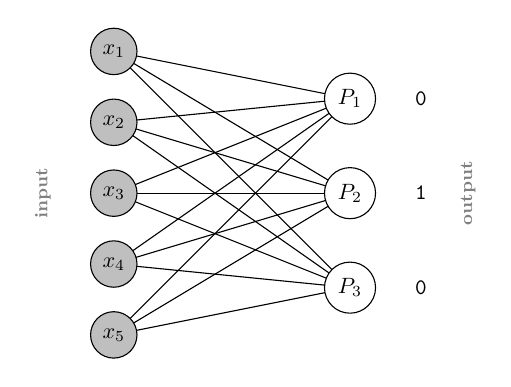
\begin{tikzpicture}[
		scale=0.6,
		every node/.style={scale=0.8}
	]

		\foreach \y in {-3,-1.5,0,1.5,3}{
			\foreach \yy in {-2,0,2}{
				\draw (-5,\y) -- (0,\yy);
			}
		}
	
		% input layer
		\foreach \y/\i in {3/1,1.5/2,0/3,-1.5/4,-3/5}{
			\node[circle,draw=black,fill=lightgray] at (-5,\y) {$x_{\i}$};
		}
		
		% rbf layer
		\foreach \y/\i in {-2/3,0/2,2/1}{
			\node[circle,draw=black,fill=white,align=center] at (0,\y) {$P_{\i}$};
		}
		\node at (1.5,2) {\texttt{0}};
		\node at (1.5,0) {\texttt{1}};
		\node at (1.5,-2) {\texttt{0}};

		\node[rotate=90,gray] at (-6.5,0) {\footnotesize \textbf{input}};
		\node[rotate=90,gray] at (2.5,0) {\footnotesize \textbf{output}};

	\end{tikzpicture}
\end{figure}
	}
\end{frame}


% What about non-linear Data Sets?
\begin{frame}{What about non-linear Data Sets?}{}
	\divideTwo{0.39}{
		\begin{itemize}
			\item Perceptrons cannot learn non-linear boundaries
			\item Remember \textit{Minsky} and \textit{Papert}
			\item What can we do?
			\begin{enumerate}
				\item Add feature mapping {\scriptsize(cf. right)}
				\item Add hidden layers \\
					{\scriptsize\highlight{(Multi-Layer Perceptrons)}}
			\end{enumerate}
	\end{itemize}
	}{0.59}{
		\begin{figure}
			\centering
			\includegraphics[scale=0.35]{10_deep_learning/02_img/rbfn}
		\end{figure}
	}
\end{frame}


% Section: Multi-Layer-Perceptrons (MLPs)
%______________________________________________________________________
\section{Multi-Layer-Perceptrons (MLPs)}
\makedivider{Multi-Layer-Perceptrons (MLPs)}


% Subsection: MLP
% --------------------------------------------------------------------------------------------------------
\subsection{Overview}

\begin{frame}{Overview: Multi-Layer Perceptron Representation}{}
	\begin{itemize}
		\item A Multi-Layer Perceptron (MLP) can approximate any continuous function arbitrarily well (universal function approximator), given enough hidden units
		\item Hidden layers of the network can learn useful feature representations
	\end{itemize}
	\begin{figure}
		\centering
		\includegraphics[scale=0.45]{10_deep_learning/02_img/mlp}
	\end{figure}
\end{frame}

\begin{frame}{Overview: Multi-Layer Perceptron Representation}{}
	\begin{itemize}
		\item An MLP with $L$ hidden layers is a function:
		\begin{itemize}
			\item $f: \mathcal{R}^n \rightarrow \mathcal{R}^m$
			\item with parameter matrices $\bm{\Theta}^{(1)}$, $\bm{\Theta}^{(2)}$, \dots, $\bm{\Theta}^{(L)}$
			\item and non-linearities $g^{(1)}$, $g^{(2)}$, \dots, $g^{(L)}$
			\item where:
			\begin{align*}
				z^{(1)} &= \bm{\Theta^{(1)}} \bm{x}\\
				z^{(2)} &= \bm{\Theta^{(2)}} g^{(1)}(\bm{z^{(1)}})\\
				\text{\dots}\\
				z^{(L)} &= \bm{\Theta^{(L-1)}} g^{(L-1)}(\bm{z^{(L-1)}})\\
				\bm{h} = g^{(L)}(\bm{z^{(L)}})
			\end{align*}
		\end{itemize}
	\end{itemize}
\end{frame}

\begin{frame}{Overview: Multi-Layer Perceptron Inference}{}
	\begin{itemize}
		\item The forward pass (prediction) of an MLP can be computed as follows:
		$$h_k(\bm{x}^{(i)}; \bm{\Theta}) = g^{(2)}\left( \sum_{l=0}^h \Theta_{kl}^{(2)} g^{(1)}\left( \sum_{j=0}^m \Theta_{lj}^{(1)} x_{j}^{(i)} \right) \right)$$
		\item This provides us with an output value for each class $k$, we could predict the class with the highest value $y = \underset{k}{\text{argmax}\,\bm{h}}$
		\item How can we obtain the optimal weights $\bm{\Theta}$?
	\end{itemize}
\end{frame}

\begin{frame}{Overview: Multi-Layer Perceptron Learning}{}
	\begin{itemize}
		\item We can optimize the parameters using gradient descent and a cost function
		\item The goal is to minimize the cost, e.\,g. $\mathcal{J}(\bm{\Theta}) = \frac{1}{2n} \sum_{i=1}^n (h_{\bm{\Theta}}(\bm{\widehat{x}}^{(i)}) - y^{(i)})^2$
		\item \texttt{Repeat until convergence \{} \\
			$\qquad \bm{\Theta}^{(t+1)} \longleftarrow \bm{\Theta}^{(t)} - \alpha \nabla_{\bm{\Theta}}
				\mathcal{J}(\bm{\Theta}^{(t)}) \quad$
			\textcolor{myblue1}{\textit{// simultaneously update all} $\theta_j$} \\
		\texttt{\}}
		\item How do we get the gradient $\nabla_{\bm{\Theta}} \mathcal{J}(\bm{\Theta})$ with respect to all weights $\bm{\Theta^{(\text{layer})}_{lj}}$?
	\end{itemize}
\end{frame}

\begin{frame}{Overview: Multi-Layer Perceptron Learning}{}
	\begin{itemize}
		\item We start by randomly initializing the network weights
		\item Do not set an initial value of 0 for all weights, as this will lead to problems in backpropagation (the gradients will all be the same), but initialize to small random numbers, e.\,g. by sampling from $\mathcal{N}(0, 0.1)$
		\item We then perform a forward pass through the network, i.\,e. make predictions on our training set
		\item Using the predictions, we compute a scalar loss value $J(\bm{\Theta})$
		\item We calculate the gradients of the loss with respect to each network parameter and update all network parameters using gradient descent
	\end{itemize}
\end{frame}


% Subsection: Backpropagation
% --------------------------------------------------------------------------------------------------------
\subsection{Backpropagation}

% Backpropagation
\begin{frame}{Backpropagation}{}\important
	\begin{itemize}
		\item In order to update the weights, we first have to perform a \highlight{forward pass}:
		\begin{align*}
			h_k(\bm{x}^{(i)}; \bm{\Theta})
				&= g^{(2)}\left( \sum_{l=0}^h \Theta_{kl}^{(2)} g^{(1)}\left( \sum_{j=0}^m \Theta_{lj}^{(1)} x_{j}^{(i)} \right) \right) \\
			z_l
				&=  g^{(1)}\left( \sum_{j=0}^m \Theta_{lj}^{(1)} x_{j}^{(i)} \right) \qquad\text{activation}
		\end{align*}
		\item $g(\cdot) \equiv$ activation function, e.\,g. sigmoid, tanh, ReLU
		\item $\bm{\Theta}$ are the network parameters (to be learned)
	\end{itemize}
\end{frame}


% Backpropagation (Ctd.)
\begin{frame}[plain]{}{}
	\bubble{0.5}{0.5}{
		\tiny This is a fully connected \\[-2mm]
		\tiny neural network
	}
	\begin{figure}
	\centering
	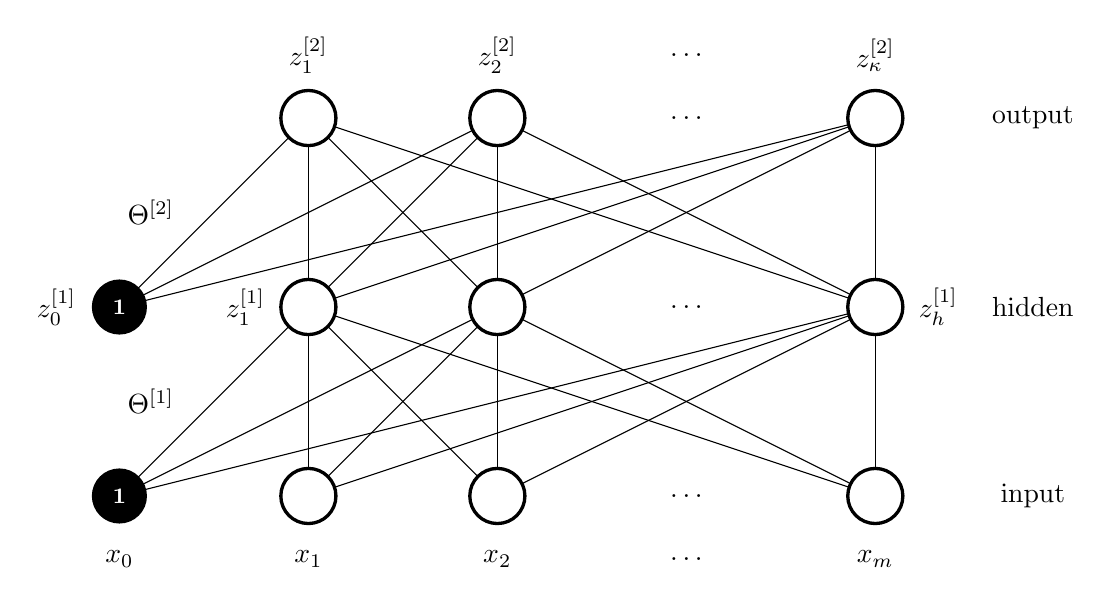
\begin{tikzpicture}[
		scale=0.8,
		b/.style={circle,fill=black,minimum width=7mm},
		n/.style={circle,draw=black,fill=white,very thick,minimum width=7mm}
	]
		
		\foreach \y in {3,6}{
			\foreach \i in {-4.5,-1.5,1.5,7.5}{
				\foreach \j in {-1.5,1.5,7.5}{
					\draw (\i, \y-3) -- (\j,\y);
				}
			}
		}
		
		% input layer
		\node[b] at (-4.5,0) {\footnotesize\textcolor{white}{\textbf{1}}};
		\node[n] at (-1.5,0) {};
		\node[n] at (1.5,0) {};
		\node at (4.5,0) {$\dots$};
		\node[n] at (7.5,0) {};

		% hidden layer
		\node[b] at (-4.5,3) {\footnotesize\textcolor{white}{\textbf{1}}};
		\node[n] at (-1.5,3) {};
		\node[n] at (1.5,3) {};
		\node at (4.5,3) {$\dots$};
		\node[n] at (7.5,3) {};

		% output layer
		\node[n] at (-1.5,6) {};
		\node[n] at (1.5,6) {};
		\node at (4.5,6) {$\dots$};
		\node[n] at (7.5,6) {};

		% input
		\node at (-4.5,-1) {$x_0$};
		\node at (-1.5,-1) {$x_1$};
		\node at (1.5,-1) {$x_2$};
		\node at (4.5,-1) {$\dots$};
		\node at (7.5,-1) {$x_m$};
		
		% output
		\node at (-1.5,7) {$z_1^{[2]}$};
		\node at (1.5,7) {$z_2^{[2]}$};
		\node at (4.5,7) {$\dots$};
		\node at (7.5,7) {$z_\kappa^{[2]}$};

		% hidden
		\node at (-5.5,3) {$z_0^{[1]}$};
		\node at (-2.5,3) {$z_1^{[1]}$};
		\node at (8.5,3) {$z_h^{[1]}$};

		% weights
		\node at (-4,1.5) {$\bm{\Theta}^{[1]}$};
		\node at (-4,4.5) {$\bm{\Theta}^{[2]}$};
		
		\node at (10,0) {\highlight{input}};
		\node at (10,3) {\highlight{hidden}};
		\node at (10,6) {\highlight{output}};
		
	\end{tikzpicture}
\end{figure}
\end{frame}


% Backpropagation (Ctd.)
\begin{frame}{Backpropagation (Ctd.)}{}\important
	\begin{itemize}
		\item Compute the network loss
		\item The loss function is given by: {\footnotesize(assume square loss: $\ell = (h_k(\bm{x}^{(i)}; \bm{\Theta}) - y_k^{(i)})^2$)}
		\begin{equation*}
			\mathcal{J}(\bm{\Theta}) = \frac{1}{n} \sum_{i=1}^n \sum_{k=1}^\kappa
				\ell(h_k(\bm{x}^{(i)}; \bm{\Theta}), y_k^{(i)})
		\end{equation*}
		\item Compute the error gradient w.\,r.\,t. $h_k(\bm{x}^{(i)}; \bm{\Theta})$:
		\begin{equation*}
			 \frac{\partial \mathcal{J}^{(i)}(\bm{\Theta})}{\partial h_k(\bm{x}^{(i)}; \bm{\Theta})}
			 	= \ell'(h_k(\bm{x}^{(i)}; \bm{\Theta}), y_k^{(i)}) \equiv \delta_k^{(i)}
		\end{equation*}
	\end{itemize}
\end{frame}


% Backpropagation (Ctd.)
\begin{frame}{Backpropagation (Ctd.)}{}\important
	\begin{itemize}
		\item Compute the weight gradient for the output layer:
		\begin{align*}
			\frac{\partial \mathcal{J}^{(i)}(\bm{\Theta})}{\partial \Theta_{kl}^{(2)}}
				&= \frac{\partial \mathcal{J}(\bm{\Theta})}{\partial h_k(\bm{x}^{(i)}; \bm{\Theta})}
					\frac{\partial h_k(\bm{x}^{(i)}; \bm{\Theta})}{\partial \Theta_{kl}^{(2)}} \\
				&= \ell'(h_k(\bm{x}^{(i)}; \bm{\Theta}), y_k^{(i)}) \cdot g'^{(2)} \left( \sum_{t=0}^h \Theta_{kt}^{(2)} z_t(\bm{x}^{(i)}) \right)
					\cdot z_l(\bm{x}^{(i)}) \\
				&= \delta_k^{(i)} \cdot g'^{(2)} \left( \sum_{t=0}^h \Theta_{kt}^{(2)} z_t(\bm{x}^{(i)}) \right) \cdot z_l(\bm{x}^{(i)})
		\end{align*}
	\end{itemize}
\end{frame}


% Backpropagation (Ctd.)
\begin{frame}{Backpropagation (Ctd.)}{}\important
	\begin{itemize}
		\item Compute the error gradient for the hidden layer:
		\begin{align*}
			\frac{\partial \mathcal{J}^{(i)}(\bm{\Theta})}{\partial z_l}
				&= \sum_{k=1}^\kappa \frac{\partial \mathcal{J}^{(i)}(\bm{\Theta})}{\partial h_k(\bm{x}^{(i)}; \bm{\Theta})}
					\frac{\partial h_k(\bm{x}^{(i)}; \bm{\Theta})}{\partial z_l} \\
				&= \sum_{k=1}^\kappa \ell'(h_k(\bm{x}^{(i)}; \bm{\Theta}), y^{(i)})
					\cdot g'^{(2)}\left( \sum_{t=0}^h \Theta_{kt}^{(2)} z_t(\bm{x}^{(i)}) \right) \cdot \Theta_{kl}^{(2)} \\
				&= \sum_{k=1}^\kappa \delta_k^{(i)} \cdot g'^{(2)} \left( \sum_{t=0}^h \Theta_{kt}^{(2)} z_t(\bm{x}^{(i)}) \right)
					\cdot \Theta_{kl}^{(2)} \equiv \widehat{\delta}_l^{(i)}
		\end{align*}
	\end{itemize}
\end{frame}


% Backpropagation (Ctd.)
\begin{frame}{Backpropagation (Ctd.)}{}\important
	\begin{itemize}
		\item Compute the weight gradient for the hidden layer:
		\begin{align*}
			\frac{\partial \mathcal{J}^{(i)}(\bm{\Theta})}{\partial \Theta_{lj}^{(1)}}
				&= \frac{\partial \mathcal{J}^{(i)}(\bm{\Theta})}{\partial z_l} \cdot g'^{(1)} \left( \sum_{t=0}^m \Theta_{jt}^{(1)} x_j^{(i)} \right) \cdot x_j^{(i)} \\
				&= \widehat{\delta}_l^{(i)} \cdot g'^{(1)} \left( \sum_{t=0}^m \Theta_{jt}^{(1)} x_j^{(i)} \right) \cdot x_j^{(i)}
		\end{align*}
		\item The weight derivatives are now used in the gradient descent update rule
	\end{itemize}
\end{frame}


% Backpropagation Example
\begin{frame}{Backpropagation Example}{}
	\begin{figure}
	\centering
	\begin{tikzpicture}[
		scale=0.8,
		b/.style={circle,fill=black,minimum width=7mm},
		n/.style={circle,draw=black,fill=white,very thick,minimum width=7mm}
	]
		
		
		
	\end{tikzpicture}
\end{figure}
\end{frame}

\begin{frame}{Remarks}{}
	\begin{itemize}
		\item As a sanity check, we can perform numeric gradient checking: Based on the fact that $f'(x) \approx \frac{1}{v} \cdot (f(x + v) - f(x))$, we can evaluate the loss function for slightly different weights and compare the difference to the gradient we computed using backprop
		\item There are a lot of hyperparameters for backprop and gradient descent (number of hidden layers, hidden layer dimensionality, activation functions, learning rate, batch size, number of training epochs, regularization, etc.) - you need to empirically find the best ones for your problem
		\item Play with some hyperparameters here: \url{https://playground.tensorflow.org}
	\end{itemize}
\end{frame}

\subsection{Activation Functions}
\begin{frame}{Sigmoid Function}{}
	\begin{itemize}
		\item $\sigma(x) = \frac{1}{1 + e^{-x}}$
		\item $\sigma'(x) = \sigma(x) (1 - \sigma(x))$
		\item Value range 0 to 1
		\item Problem: Gradient can become very small (vanishing gradient), in contrast to large gradients it's not clear how to clip the gradient on the lower end
		\item Problem: Output is not zero-centered (sigmoid output is always positive, gradients will be all positive or all negative which makes optimization harder)
	\end{itemize}
\end{frame}

\begin{frame}{Sigmoid Function}{}
	\begin{itemize}
		\item \textit{Convergence is usually faster if the average of each input variable over the training set is close to zero. To see this, consider the extreme case where all the inputs are positive. Weights to a particular node in the first weight layer are updated by an amount proportional to $\delta$x where $\delta$ is the (scalar) error at that node and x is the input vector (see equations (5) and (10)). When all of the components of an input vector are positive, all of the updates of weights that feed into a node will have the same sign (i.e. sign($\delta$)). As a result, these weights can only all decrease or all increase together for a given input pattern. Thus, if a weight vector must change direction it can only do so by zigzagging which is inefficient and thus very slow.} - Yann LeCun et al., Efficient BackProp, 1998 (\url{http://yann.lecun.com/exdb/publis/pdf/lecun-98b.pdf})
	\end{itemize}
\end{frame}

\begin{frame}{tanh}{}
	\begin{itemize}
		\item $\tanh(x) = \frac{e^x - e^{-x}}{e^x + e^{-x}}$
		\item $\tanh'(x) = 1 - \tanh(x)^2$
		\item Value range -1 to 1
		\item Zero-centered
		\item Still suffers from the vanishing gradient problem
	\end{itemize}
\end{frame}

\begin{frame}{Rectified Linear Unit (ReLU)}{}
	\begin{itemize}
		\item $ReLU(x) = max(0,x)$
		\item $ReLU'(x) = \begin{Bmatrix}
0 & x<0 \\
1 & x>0 \\
\end{Bmatrix}$
	\end{itemize}
	\begin{figure}
		\centering
		\begin{tikzpicture}[scale=0.6]
		\begin{axis}[domain=-3:5]
		\addplot+[mark=none,red,domain=-3:0] {0};
		\addplot+[mark=none,red,domain=0:5] {x};
		\end{axis}
		\end{tikzpicture}
	\end{figure}
\end{frame}

\begin{frame}{Rectified Linear Unit (ReLU)}{}\important
	\begin{itemize}
		\item ReLU does not lead to vanishing gradients
		\item ReLU is very efficient to compute
		\item Use ReLU as the hidden layer activation function!
		\item But: Pay attention to the initialization of your parameters to avoid \textit{"dying ReLUs"} (parameter settings where single neurons will always output 0)
	\end{itemize}
\end{frame}

\begin{frame}{Softmax}{}
	\begin{itemize}
		\item $softmax_i(x) = \frac{e^{x_i}}{\sum_{j=1}^K e^{x_j}}$
		\item $\frac{\partial s_i}{\partial a_j} = \begin{Bmatrix}
s_i (1 - s_j) & i = j \\
-s_i \cdot s_j & i \ne j \\
\end{Bmatrix}$
		\item Used to squash the last layer's activations into a probability distribution
	\end{itemize}
\end{frame}

% Section: Further Network Architectures
%______________________________________________________________________
\section{Further Network Architectures}
\makedivider{Further Network Architectures}

% Subsection: Convolutional Neural Networks
% --------------------------------------------------------------------------------------------------------
\subsection{Convolutional Neural Networks}

\begin{frame}{Convolutional Neural Networks}{Motivation}
	\begin{itemize}
		\item A large fully-connected MLP network can have a lot of parameters $\rightarrow$ it might be too complex / overfit or be computationally inefficient for some tasks
		\item For some problems the input position may not matter in every case (e.\,g. when classifying emails as spam or not spam, we don't care if the word \textit{the} is at input position 3 or 5)
		\item The MLP always needs a fixed-size input vector - but we might have variable-size input data (e.\,g. images in different resolutions, text sequences of different lengths, etc.)
	\end{itemize}
\end{frame}

\begin{frame}{Convolutional Neural Networks}{Idea}
	\begin{itemize}
		\item \textit{"A convolutional neural network is designed to identify indicative local predictors in a large structure, and combine them to produce a fixed size vector representation of the structure, capturing these local aspects that are most informative for the prediction task at hand."} - Yoav Goldberg
	\end{itemize}
\end{frame}

\begin{frame}{Convolutional Neural Networks}{Representation}
	\begin{itemize}
		\item A CNN usually consists of multiple convolutional layers
		\item A convolutional layer consists of a convolution (a.k.a. filter), a non-linear activation function and a pooling operation
		\item Pooling extracts the most important features independent of their input position
	\end{itemize}
\end{frame}

\begin{frame}{Convolutional Neural Networks}{Representation}
	\begin{itemize}
		\item The convolution operation: $$(f \star g)[i] = \sum_{w=-W}^W f[i-w] g[w]$$\vspace{-0.3cm}
		\begin{itemize}
			\item $\star$ is the convolution operator,
			\item $f$ is the input to the convolutional layer,
			\item $i$ is the current position in the input,
			\item $W$ is the filter size / window size,
			\item $g$ is the filter (a.k.a. \textit{kernel})
		\end{itemize}
	\end{itemize}
\end{frame}

\begin{frame}{Convolutional Neural Networks}{Representation}
	\begin{itemize}
		\item The convolution operation: $(f \star g)[i] = \sum_{n=-N}^N f[i-n] g[n]$
		\item We stride a filter across the input data (e.\,g. image pixels) with a certain stride size and multiply the input with the filter weights at each local position
	\end{itemize}
	\begin{figure}
		\centering
		\includegraphics[scale=0.90]{10_deep_learning/02_img/flatconvolution}
	\end{figure}
\end{frame}

\begin{frame}{Convolutional Neural Networks}{Representation}
	\begin{itemize}
		\item The outputs of the convolutions are passed through non-linear activation functions
		\item Pooling is applied to extract only the most important activations:
		\begin{itemize}
			\item If $c_1, c_2, \dots, c_N \in \mathcal{R}$ are the outputs of the convolution, a \textit{max pooling} operation will output: $\underset{i}{\text{max}}\, c_i$
		\end{itemize}
		\item There are no parameters / weights involved in the pooling
	\end{itemize}
\end{frame}

\begin{frame}{Convolutional Neural Networks}{Remarks}
	\begin{itemize}
		\item Usually many (hundreds or thousands) filters are applied simultaneously
		\item We need to choose the number and size of filters, the stride (step-size) with which to slide them over the input, the activation functions, the pooling (max, $k$-max, mean)
		\item Multiple convolutional layers can be applied subsequently to extract useful structures from the data (e.\,g. detecting edges, substructures)
		\item Sparse connectivity and parameter-sharing make CNNs very efficient, computation can be parallelized
	\end{itemize}
\end{frame}

% Convolution Animation
\begin{frame}{Convolution Animation}{}
	\begin{figure}
		\centering
		\animategraphics[autoplay,loop,height=5.5cm]{2.5}
			{10_deep_learning/02_img/convolution_animation/}{0}{45}
	\end{figure}
\end{frame}

% Subsection: Recurrent Neural Networks
% --------------------------------------------------------------------------------------------------------
\subsection{Recurrent Neural Networks}

% RNN Overview
\begin{frame}{Recurrent Neural Networks}{Overview}
	\begin{itemize}
		\item Recurrent Neural Networks (RNNs) can be used to process sequences\newline (e.\,g. for sequence labelling tasks like named entity recognition, for sequence transduction tasks like machine translation, for sequence classification, etc.)
		\item They are similar to feed-forward networks, but have a recurrent loop in the computational graph
	\end{itemize}
	\begin{figure}
		\centering
		\includegraphics[scale=0.25]{10_deep_learning/02_img/rnn}
	\end{figure}
\end{frame}

\begin{frame}{Recurrent Neural Networks}{Representation}
	\begin{align*}
		\bm{h}_t &= \sigma_h(\bm{U} \bm{x} + \bm{V} \bm{h}_{t - 1} + \bm{b}_h)\\
		\bm{o_t} &= \sigma_o(\bm{W} \bm{h_t} + \bm{b}_o)
	\end{align*}
	\begin{figure}
		\centering
		\includegraphics[scale=0.25]{10_deep_learning/02_img/rnn}
	\end{figure}
\end{frame}

\begin{frame}{Recurrent Neural Networks}{Extensions}
	\begin{itemize}
		\item Bi-directionality: Run the RNN from left-to-right and right-to-left and concatenate the hidden states $\overset{\rightarrow}{h_t}$ and $\overset{\leftarrow}{h_t}$ for both directions
		\item Gating: Gated Recurrent Units (GRUs) and Long-Short Term Memory (LSTM) Networks add additional parameters to RNNs to better control what is stored in the hidden state $h$ and to prevent vanishingly small gradients for long sequences
		\item Skip-connections through time
		\item Attention (re-expressing inputs and outputs in terms of a weighted combination with the other inputs)
	\end{itemize}
\end{frame}

\begin{frame}{Recurrent Neural Networks}{Extensions}
	\begin{itemize}
		\item Long-Short Term Memory Network (Hochreiter, Schmidhuber, 1997):
		\begin{itemize}
			\item Input gate $\bm{i}_t = \sigma(\bm{W_i} \bm{x}_t + \bm{U}_i \bm{h}_{t-1})$
			\item Forget gate $\bm{f}_t =\sigma(\bm{W_f} \bm{x}_t + \bm{U}_f \bm{h}_{t-1})$
			\item Output gate $\bm{o}_t =\sigma(\bm{W_o} \bm{x}_t + \bm{U}_o \bm{h}_{t-1})$
			\item New memory cell $\overset{\sim}{\bm{c}_t} = \tanh(\bm{W}_c \bm{x}_t + \bm{U}_c \bm{h}_{t-1})$
			\item Final memory cell $\bm{c}_t = \bm{f}_t \odot \bm{c}_{t-1} + \bm{i}_t \odot \overset{\sim}{\bm{c}_t}$
			\item Final hidden state $\bm{h}_t = \bm{o}_t \odot \tanh(\bm{c}_t)$
		\end{itemize}
		\item $\sigma$ denotes the sigmoid activation function on this slide, $\odot$ is element-wise mutliplication (a.k.a. Hadamard product)
	\end{itemize}
\end{frame}

\begin{frame}{Recurrent Neural Networks}{Extensions}
	\begin{itemize}
		\item Long-Short Term Memory Network (Hochreiter, Schmidhuber, 1997):
	\end{itemize}
	\begin{figure}
		\centering
		\includegraphics[scale=0.50]{10_deep_learning/02_img/lstm}
	\end{figure}
\end{frame}


% Section: Wrap-Up
%______________________________________________________________________
\section{Wrap-Up}
\makedivider{Wrap-Up}

% Subsection: Summary
% --------------------------------------------------------------------------------------------------------
\subsection{Summary}

% Summary
\begin{frame}{Summary}{}
	\begin{itemize}
		\item Neural Networks are powerful models for pattern recognition
		\item The Perceptron can classify all training examples correctly iff the training data is linearly separable
		\item Multi-Layer Perceptrons are universal function approximators
		\item Backpropagation is a recursive procedure based on the chain rule of calculus to obtain the gradients for neural network learning
		\item Different neural network architectures like CNNs and RNNs exist for solving different kinds of problems
	\end{itemize}
\end{frame}


% Subsection: Self-Test Questions
% --------------------------------------------------------------------------------------------------------
\subsection{Self-Test Questions}

% Self-Test Questions
\begin{frame}{Self-Test Questions}{}\important
	\begin{enumerate}
		\item What is the relation between neural networks and logistic regression?
		\item What is a perceptron? Which problems can it solve and which not?
		\item Why do we often use multiple layers used instead of a simple Perceptron?
		\item How does backpropagation work? How does a neural network learn?
		\item What are advantages and disadvantages of using neural networks?
		\item What are CNNs and RNNs? For which tasks are they suitable?
	\end{enumerate}
\end{frame}


% Subsection: Lecture Outlook
% --------------------------------------------------------------------------------------------------------
\subsection{Lecture Outlook}

\begin{frame}{What's next...?}{}
	\makeoverview{8}
\end{frame}


% Subsection: Recommended Literature and further Reading
% --------------------------------------------------------------------------------------------------------
\subsection{Recommended Literature and further Reading}

% Literature
%______________________________________________________________________
\begin{frame}{Recommended Literature and further Reading}{}
	\footnotesize
	\begin{thebibliography}{2}
		\literature{book}{Goodfellow.2016}{[1] Deep Learning}
			{Ian Goodfellow et al. MIT Press. 2016.}{$\rightarrow$ \href{
				http://www.deeplearningbook.org/
			}{\linkstyle{Link}}, cf. chapters 6 \textit{Deep Feedforward Networks}, especially chapter 6.5}
	
		\literature{book}{Bishop.2006}{[2] Pattern Recognition and Machine Learning}
			{Christopher Bishop. Springer. 2006.}{$\rightarrow$ \href{
				http://users.isr.ist.utl.pt/~wurmd/Livros/school/Bishop\%20-\%20Pattern\%20Recognition\%20And\%20Machine\%20Learning\%20-\%20Springer\%20\%202006.pdf
			}{\linkstyle{Link}}, cf. chapter 5 \textit{Neural Networks}, especially chapter 5.3}

		\literature{online}{Saunderson.2017}{[3] Backpropagation calculus}
			{Grant Saunderson. YouTube. 2017.}{$\rightarrow$ \href{
				https://www.youtube.com/watch?v=tIeHLnjs5U8
			}{\linkstyle{Link}}}

	\end{thebibliography}
\end{frame}

\begin{frame}{Recommended Literature and further Reading}{}
	\footnotesize
	\begin{thebibliography}{2}
		\literature{online}{Ng.2019}{[4] Simple Backpropagation in NumPy}
			{Andrew Ng et al. Stanford CS229. 2019.}{$\rightarrow$ \href{
				http://cs229.stanford.edu/notes/backprop.py
			}{\linkstyle{Link}}}

	\end{thebibliography}
\end{frame}


% Thank you
%______________________________________________________________________
\makethanks

\end{document}